\section{Theorie}
\label{sec:Theorie}
\subsection{Komplexe Widerstände}
Bevor die Brückenschaltungen im Einzelnen betrachtet werden, muss zwischen verschiedenen Formen von elektrischen Widerständen -- 
auch \textit{Impedanzen} -- unterschieden werden. 

Neben den ohmschen Widerständen $R$ sorgen auch Spulen mit der Induktivität $L$ und Kondensatoren mit der Kapazität $C$, 
die sich mit im Stromkreis befinden, für eine Veränderung des Strom- und Spannungsverhalten. 
Der ohmsche Widerstand sorgt für einen Spannungsabfall von 
\begin{equation}
    U=RI .
    \label{eqn:ohm}
\end{equation}
Kondensatoren und Spulen hingegen bewirken zusätzlich eine Phasenverschiebung des Wechselstroms und der Wechselspannung,
die den Stromkreis betreiben. 
In der reellen Schreibweise mit trigonometrischen Funktionen recht kompliziert, vereinfacht sich die Darstellung dessen 
mit komplexen Zahlen: 
Ohmsche sowie induktive und kapazitive Widerstände werden zu einer komplexwertigen Impedanz zusammengefasst. 
Dabei stellen letztere beiden den Imaginäranteil dar, wodurch die Phasenverschiebung algebraisch umgesetzt wird. 
Da sie in dem Sinne keinen effektiven Spannungsabfall bewirken, sind sie auch unter dem Namen \textit{Scheinwiderstand} geläufig.
Somit hat die Impedanz $Z$ von den drei in Reihe geschalteten Widerständen die Form 
\begin{equation}
    Z = R + \symup{i}\omega L - \symup{i}\frac{1}{\omega C} ,
    \label{eqn:impedanz}
\end{equation}
wobei $\omega$ die Kreisfrequenz der angelegten Wechselspannung $\tilde{U} = \hat{U} \symup{e}^{\symup{i}\omega t}$ ist.
Mit der komplexen Impedanz kann wie mit dem ohmschen Widerstand in \eqref{eqn:ohm} die Spannung und der Strom berechnet werden. 

\subsection{Die Kirchhoff'schen\footnote{\textit{nach Gustav Robert Kirchhoff (1824 - 1887), deutscher Physiker}} Gesetze}
Das erste Gesetz, ebenfalls unter der Knotenregel bekannt, leitet sich aus der Ladungserhaltung ab. 
An einem Knoten in einem Stromkreis muss die Summe der zufließenden Ströme gleich der der abfließenden sein. 
Definiert man eine entsprechende Vorzeichenregelung (z.B. alle abfließenden Ströme sind positiv, alle zufließenden negativ) 
erhält man den Ausdruck: 
\begin{equation}
    \sum_k I_k=0 .
    \label{eqn:kirchhoff1}
\end{equation}

Das zweite Gesetz beruft sich auf die Energieerhaltung und die Existenz eines eindeutigen elektrischen Potentials. 
Als Folgerung daraus ergibt sich die sogenannte Maschenregel, die 
\begin{equation}
    \sum_k U_k=0
    \label{eqn:kirchhoff2}
\end{equation}
innerhalb eines geschlossenen Leiters -- also einer Masche -- postuliert. 
Dabei sind die Spannungsquellen und -abfälle $U_k$ jeweils mit einem entsprechenden Vorzeichen versehen, je nachdem, ob sie 
in gleicher oder verschiedener Richtung gepolt sind. 

\subsection{Brückenschaltungen} 
Das Konzept der Brückenschaltung basiert auf den Kirchhoff'schen Gesetzen.
Mit einer Parallelschaltung und den vorliegenden Gesetzen kann bei bekannten Widerständen ein unbekannter Widerstand bestimmt werden.
Diese Schaltungen werden wegen ihrer hohen Genauigkeit in der Messtechnik häufig eingesetzt.
Dabei ist die Auflösung davon abhängig, wie gut die Bauelemente bekannt sind, wie hoch ihre Ungenauigkeiten sind und wie hoch die Speisespannung ist.
In Abb. \ref{fig:allg_schalt} ist der konzeptionelle Aufbau einer Brückenschaltung zu sehen.

\begin{figure}
    \centering
    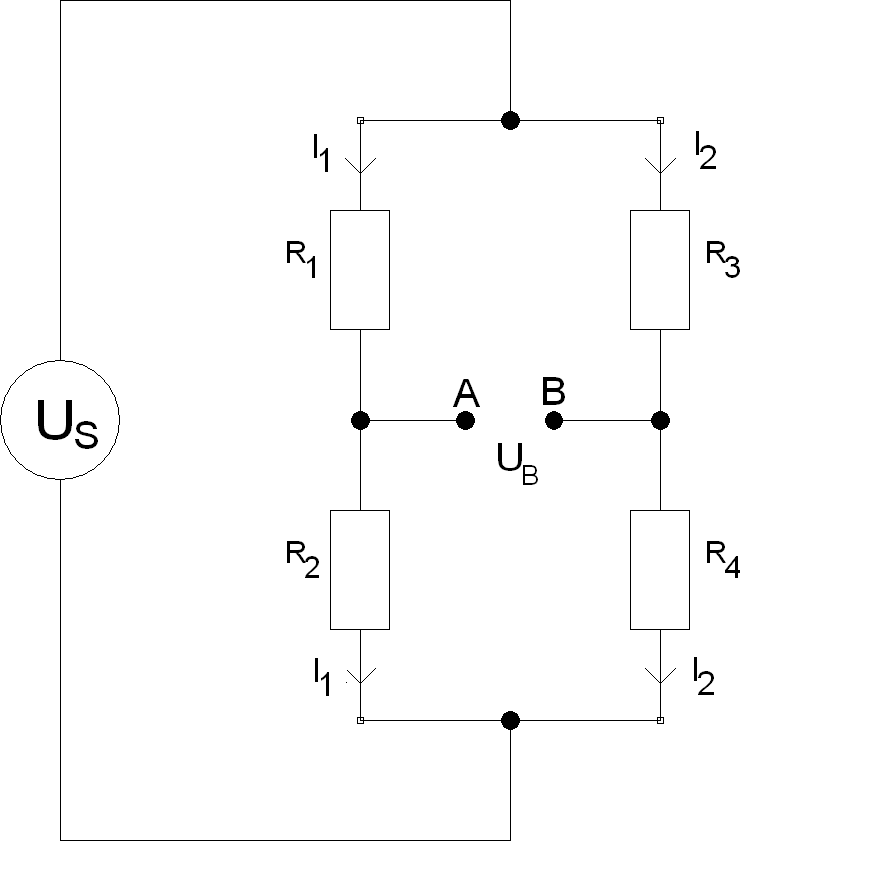
\includegraphics[width=0.5\textwidth]{plots/allgBrSchalt.png} %Abbildung ändern (I3, I4)
    \caption{Eine allgemeine Brückenschaltung.}
    \label{fig:allg_schalt}
\end{figure}

Zwischen den Punkten A und B kann eine Spannung gemessen werden, welche als Brückenspannung $U_B$ bezeichnet wird.
Mit der sogenannten Nullmethode können bspw. die Widerstände 2, 3 und 4 derart variiert werden, sodass die Brückenspannung $U_B = 0$ wird.
So kann mit der Bekanntheit der drei genannten Widerstände $R_1$ berechnet werden.

Über die Maschenregel \ref{eqn:kirchhoff1} gilt
\begin{equation*}
    M_1: U = R_1I_1 - R_3I_2.
\end{equation*}
Außerdem gilt
\begin{equation*}
    M_2: U = R_2I_1 - R_4I_2.
\end{equation*}

Daraus folgt, dass
\begin{equation*}
    U_B = I_1\frac{R_2R_3 - R_1R_4}{R_3 + R_4}.
\end{equation*}

Die Speisespannung können wir über die Maschenregel ausdrücken als 
\begin{equation*}
    U_S = R_1I_1 + R_2I_1.
\end{equation*}

Somit erhalten wir eine Gleichung, welche die Brückenspannung in Abhängigkeit von den Widerständen und der Speisespannung angibt.
\begin{equation}
    U = \frac{R_2R_3 - R_1R_4}{(R_3 + R_4)(R_1 + R_2)}U_S
    \label{eqn:verhmitspeise}
\end{equation}
Folgt nun, dass der Zähler des Ausdrucks Null wird, so verschwindet $U_B$ und ist nur noch von den Widerstandsverhältnissen und nicht mehr
von der Eingangsspannung $U_S$ abhängig. 
\begin{equation}
    R_2R_3 = R_1R_4
    \label{eqn:abgeglichenOhm}
\end{equation}
Auf diesem Prinzip bauen alle Brückenschaltungen auf. %ist das so?
$U_B$ ist hier immer noch proportional zu $U_S$, weswegen eine höhere Messgenauigkeit erreicht wird, wenn 
die Speisespannung hoch ist.
Eine Brückenschaltung, dessen Brückenspannung Null ist, nennt man abgeglichen.

\subsubsection{Wheatstone'sche\footnote{\textit{Charles Wheatstone (1802 - 1875), britischer Physiker}} Brückenschaltung}
Die Wheatstone'sche Brückenschaltung nutzt ohmsche Widerstände, um einen unbekannten Widerstand $R_x$ zu ermitteln.
Hier wird für die eine Seite der Parallelschaltung ein Potentiometer verwendet, sodass das Widerstandsverhältnis $R_3$ zu $R_4$ stufenlos eingestellt werden kann, 
bis die Brückenspannung Null wird.
Da $R_2$ bei dieser Schaltung fest und bekannt ist, errechnet sich der gesuchte Widerstand durch
\begin{equation}
    R_x = \frac{R_2R_3}{R_4}.
    \label{eqn:wheatstone}
\end{equation}
\pagebreak
\begin{figure}
    \centering
    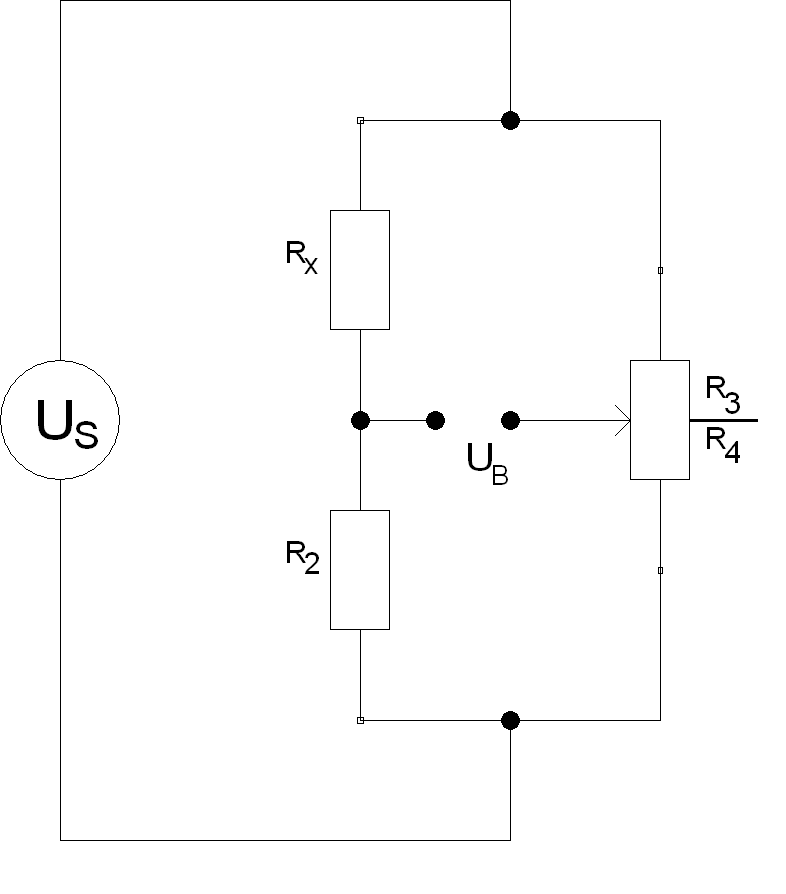
\includegraphics[width=0.5\textwidth]{plots/wheatstone.png}
    \caption{Die Wheatstone'sche Brückenschaltung.}
    \label{fig:wheatstone}
\end{figure}

\subsubsection{Kapazitätsmessbrücke}
Impedanzen, die aus einem Wirkwiderstand und einem Blindwiderstand bestehen, werden mit einem Real- und Imaginäranteil angegeben, die zusammen als
komplexe Zahl angegeben werden. Dabei gibt es zwei grundlegende Bauelemente, zwischen denen man unterscheidet.
Die Impedanz eines Kondensators C und einer Spule L, wobei
\begin{equation*}
    Z_R = R
    \quad\mathrm{,}\quad
    Z_L = i\omega L
    \quad\mathrm{und}\quad 
    Z_C = -\frac{i}{\omega C}  .
\end{equation*}

Bekanntlich sind zwei komplexe Zahlen gleich, wenn ihre Real- und Imaginäranteile gleich sind.
Es folgen damit aus \ref{eqn:abgeglichenOhm}
\begin{equation*}
    Z_2Z_3 = Z_1Z_4
\end{equation*} zwei Gleichungen
\begin{equation}
    x_2x_3 - y_2y_3 = x_1x_4 - y_1y_4
\end{equation}
und
\begin{equation}
    x_2y_3 + x_3y_2 = x_1y_4 + x_4y_1  .
\end{equation}
Hierbei sind x und y Real- und Imaginäranteil der Impedanzen $Z_1$ bis $Z_4$.
Es müssen bei einer Kapazitätsmessbrücke also nicht nur die Wirkwiderstände, also die ohm'schen Anteile verschwinden, sondern 
auch die Blindwiderstände, also der Phasenanteil.
Reale Kondensatoren speichern nicht nur Energie, sondern weisen auch einen geringen ohm'schen Widerstand auf. In einem Schaltbild
wir so ein realer Kondensator also als ein ohm'scher Widerstand und einem in Reihe geschalteten Kondensator dargestellt.
Die Brückenschaltung kann genau wie bei der Wheatstone'schen Brücke aufgebaut werden.
\begin{figure}
    \centering
    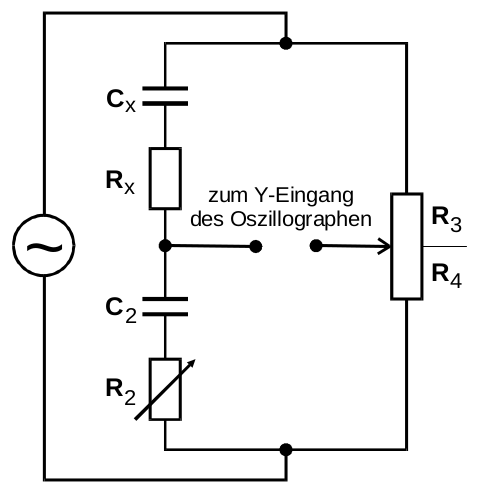
\includegraphics[width=0.5\textwidth]{plots/kapazität.png}
    \caption{Eine Kapazitätsmessbrücke.}
    \label{fig:Kapazität}
\end{figure}
Nach den zuletzt genannten Gleichungen ergibt sich
\begin{equation*}
    y_3 = y_4 = 0
    \quad\mathrm{,}\quad
    y_1 = \frac{-1}{\omega C_x}
    \quad\mathrm{und}\quad 
    y_2 = \frac{-1}{\omega C_2} .
\end{equation*}
und damit zusätzlich zu \ref{eqn:abgeglichenOhm} auch noch 
\begin{equation}
    C_x = C_2\frac{R_4}{R_3} .
    \label{eqn:abgeglKapaz}
\end{equation}
Es muss also nur noch ein weiterer Widerstand $R_2$ variiert werden, welcher unabhängig von dem $R_3R_4$-Potentiometer ist.

\subsubsection{Induktionsmessbrücke}

\begin{figure}
    \centering
    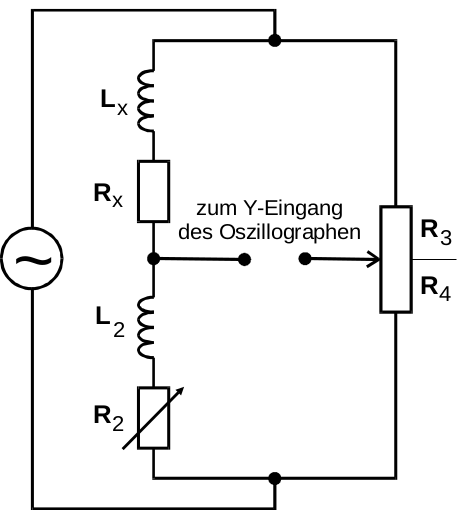
\includegraphics[width=0.5\textwidth]{plots/induk.png}
    \caption{Eine Induktivitätsmessbrücke.}
    \label{fig:induk}
\end{figure}

Eine Induktionsmessbrücke verhält sich analog zur Kapazitätsmessbrücke.
Lediglich \ref{eqn:abgeglKapaz} ändert sich zu 
\begin{equation}
    L_x = L_2\frac{R_4}{R_3} .
    \label{eqn:abgeglInduk}  
\end{equation}

Da jedoch gerade bei niedrigen Frequenzen die Wirkanteile der Spulen zu große Verluste aufweisen, greift man oft auf eine Kapazität zurück.
Solch eine Schaltung ist dann die Maxwell-Brücke.

\subsubsection{Maxwell\footnote{\textit{James Clerk Maxwell (1831 - 1879), britischer Physiker}}-Brücke}
In dieser Schaltung werden die Widerstände $R_3$ und $R_4$ variiert.
Unbekannt sind $L_x$ und $R_x$.
\begin{figure}
    \centering
    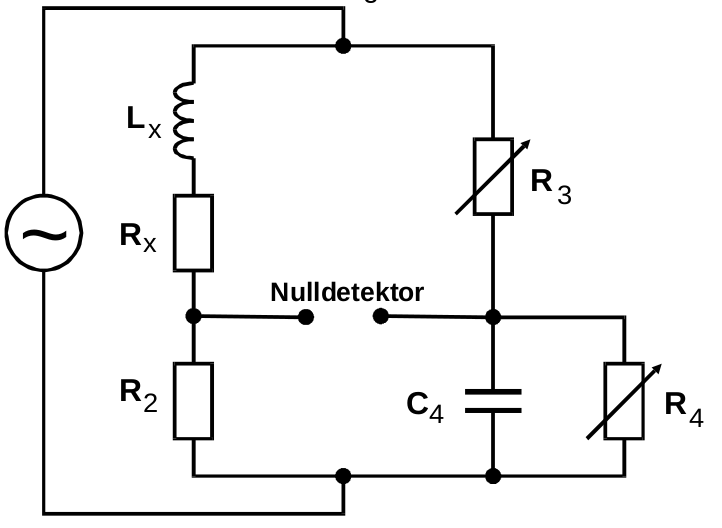
\includegraphics[width=0.5\textwidth]{plots/maxwell.png}
    \caption{Die Maxwell-Brücke.}
    \label{fig:maxell}
\end{figure}
Es ist 
\begin{equation*}
    Z_1 = R_x + i\omega L_x .
\end{equation*}
Mit den Abgleichbedingungen \ref{eqn:abgeglInduk} und \ref{eqn:abgeglichenOhm} ergibt sich die Gleichung
\begin{equation*}
    R_xR_4(1+\omega ²C_4²R_4²) = R_2R_3(1+\omega ²C_4²R_4²) .
\end{equation*}

Daraus folgt wieder \ref{eqn:abgeglichenOhm}, aber auch 
\begin{equation}
    L_x = R_2R_3C_4  .
    \label{eqn:abgeglMaxwell}
\end{equation}

Es ist sofort erkennbar, dass die Frequenzabhängigkeit im abgeglichenen Zustand verschwindet.
Außerdem werden somit die niederfrequenten Störeffekte umgangen.

\subsubsection{Wien-Robinson-Brücke\footnote{\textit{Max Wien (1866 - 1938). Der Oszillator wurde erstmals von William Hewlett und David Packard gebaut und vermarktet. Für diesen Zweck gründeten sie Hewlett-Packard, wodurch Wiens Erfindung als Fundament der Firma diente.}}}
Anders zu den anderen Brückenschaltungen ist die Wien-Robinson-Brückenschaltung frequenzabhängig.
\begin{figure}
    \centering
    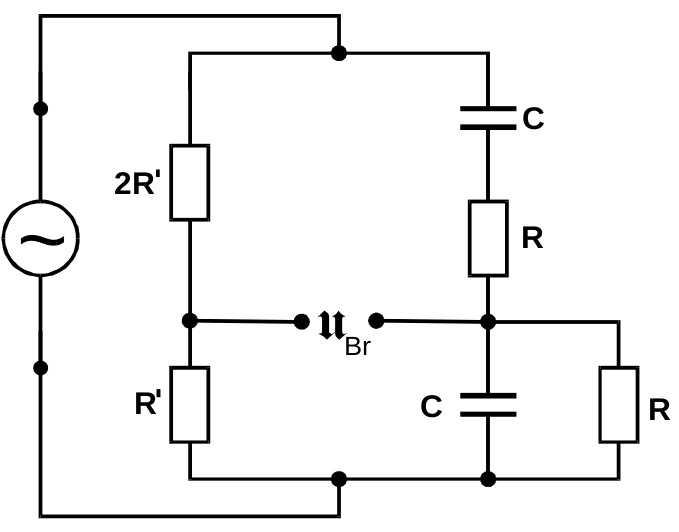
\includegraphics[width=0.5\textwidth]{plots/wien.png}
    \caption{Wien-Robinson-Brücke.}
    \label{fig:wien}
\end{figure}
Aus \ref{eqn:verhmitspeise} ergibt sich für Impedanzen
\begin{equation*}
    U = \frac{Z_2Z_3 - Z_1Z_4}{(Z_3 + Z_4)(Z_1 + Z_2)}U_S  .
\end{equation*}
Nach ein paar Doppelbrüchen kann das Verhältnis von Brücken- zu Speisespannung als Funktion der Frequenz angegeben werden.
Daraus folgt das Betragsquadrat
\begin{equation}
    \biggl|\frac{U_B}{U_S}\biggr|² = \frac{(\omega ²R²C² - 1)²}{9[(1-\omega ²R²C²)² + 9\omega ²R²C²]}  .
\end{equation}
Daraus folgt wieder, dass die Brückenspannung genau dann verschwindet, wenn 
\begin{equation*}
    \omega_0 = \frac{1}{RC} .
\end{equation*}
Die Gleichung wird dann zu 
\begin{equation}
    \biggl|\frac{U_B}{U_S}\biggr|² = \frac{1}{9}\frac{\biggl(\frac{\omega}{\omega_0}-1\biggr)²}{\biggl(1-\frac{\omega}{\omega_0}²\biggr)² + 9\frac{\omega}{\omega_0}²} .
    \label{eqn:wienfinal}
\end{equation}
An \ref{eqn:wienfinal} ist ersichtlich, dass die Schaltung einem Filter ähnelt, welcher um die Kreisfrequenz $\omega_0$ Schwingungen entfernt.
Es schwächt alle naheliegenden Schwingungen ab.